\subsection{Présentation générale}

\begin{definition}
On appelle \tdef{lentille sphérique} tout \imp{système optique centré} constistant en la succession de deux dioptres sphériques (l'axe optique passe alors par les centres de ceux-ci) ou bien d'un dioptre plan et d'un dioptre sphérique.
\end{definition}

\begin{vocabulaire}
On distingue deux grandes catégories de lentilles :
\begin{itemize}
\item les \tdef{lentilles convergentes}, plus épaisses au centre que sur les bords :

\begin{figure}[H]
\begin{center}
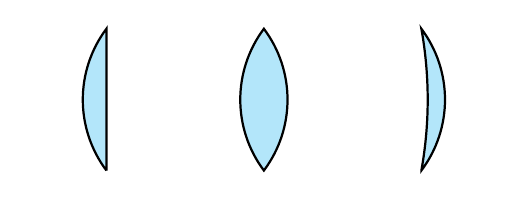
\begin{tikzpicture}[thick]
\path (-3,0) -- (3,0); % Pour la bounding box

\draw [xshift=-2cm, fill=cyan!30!white] (0,-0.9) -- (0,0.9) arc (143.1301:216.8699:1.5) -- cycle;
\draw [fill=cyan!30!white] (0,0.9) arc (36.8699:-36.8699:1.5) arc (216.8699:143.1301:1.5) -- cycle;
\draw [xshift=2cm, fill=cyan!30!white]  (0,-0.9) arc (-36.8699:36.8699:1.5) arc (10.204:-10.204:5.08) -- cycle;
\end{tikzpicture}
\end{center}
\end{figure}

\item les \tdef{lentilles divergentes}, plus épaisses sur les bords qu'au centre :

\begin{figure}[H]
\begin{center}
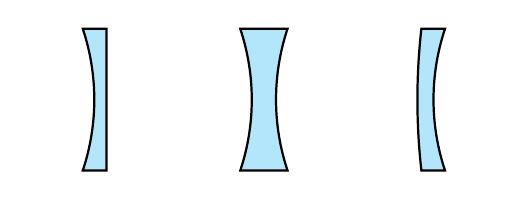
\begin{tikzpicture}[thick]
\path (-3,0) -- (3,0); % Pour la bounding box

\draw [xshift=-2cm, fill=cyan!30!white] (0,-0.9) -- (-0.3,-0.9) arc (-18.4349:18.4349:2.846) -- (0,0.9) -- cycle;
\draw [fill=cyan!30!white] (-0.3,-0.9) arc (-18.4349:18.4349:2.846) -- (0.3,0.9) arc (161.5651:198.4349:2.846) -- cycle;
\draw [xshift=2cm, fill=cyan!30!white] (0.3,-0.9) arc (198.4349:161.5651:2.846) -- (0,0.9) arc (173.58121:186.41879:8.05) -- cycle;
\end{tikzpicture}
\end{center}
\end{figure}
\end{itemize}
\end{vocabulaire}

\begin{propriete}
Une \imp{lentille sphérique}, schématisée ci-dessous :

\begin{figure}[H]
\begin{center}
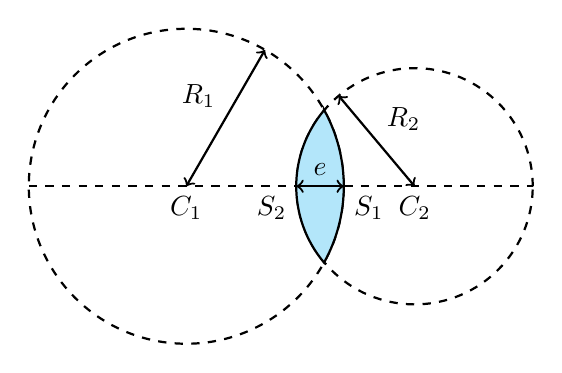
\begin{tikzpicture}[thick]
\coordinate (C1) at (-1.7,0);
\coordinate (C2) at (1.2,0);
\coordinate (S1) at (0.3,0);
\coordinate (S2) at (-0.3,0);

\draw [dashed] (C1) circle [radius=2];
\draw [dashed] (C2) circle [radius=1.5];

\draw [dashed] (-3.7,0) -- (2.7,0);

\node [below] at (C1) {$\point{C}_1$};
\node [below] at (C2) {$\point{C}_2$};

\node [below right] at (S1) {$\point{S}_1$};
\node [below left]  at (S2) {$\point{S}_2$};

\draw [<->] (C1) -- node [above left]  {$R_1$} +(60:2cm);
\draw [<->] (C2) -- node [above right] {$R_2$} +(130:1.5cm);

\draw [fill=cyan!30!white] (0.05,0.97) arc (28.999:-28.999:2) arc (220.1469:139.8531:1.5) -- cycle;

\draw [<->] (S1) -- node [above] {$e$} (S2);
\end{tikzpicture}
\end{center}
\end{figure}

\noindent est dite \tdef{mince} (ou \tdef{\abr{lms}}) lorsque son épaisseur $e$ est très petite à la fois devant les rayons de courbure $R_1$ et $R_2$ des dioptres qui la délimitent, et devant leur différence :

\begin{center}
\begin{itemize*}[itemjoin=\qquad]
\item $ e \ll R_1$
\item $ e \ll R_2$
\item $ e \ll \abs{R_1 - R_2}$
\end{itemize*}
\end{center}

\noindent Dans ce cas, $\point{O} \simeq \point{S}_1 \simeq \point{S}_2$ est appelé \tdef{centre de la lentille}.
\end{propriete}


\begin{remarque}
On schématisme une \abr{lms} différemment selon qu'elle est convergente ou non :

\begin{figure}[H]
\begin{center}
\begin{tikzpicture}[thick, use optics]
\coordinate (O1) at (-3,0);
\coordinate (O2) at (3,0);

% Left

\draw (O1) +(-2.5,0) -- +(2.5,0) node [right] {$\droite{\Delta}$};

\node[lens, lens type=converging, object height=2.4cm] (L1) at (O1) {};
\node [below=0.2] at (L1.south) {\abr{lms} convergente};

\node [below left] at (O1) {$\point{O}$};


% Right

\draw (O2) +(-2.5,0) -- +(2.5,0) node [right] {$\droite{\Delta}$};

\node[lens, lens type=diverging, object height=2.4cm] (L2) at (O2) {};
\node [below=0.2] at (L2.south) {\abr{lms} divergente};

\node [below left] at (O2) {$\point{O}$};
\end{tikzpicture}
\end{center}
\end{figure}
\end{remarque}



\subsection{Stigmatisme et aplanétisme}

\begin{propriete}[admis]
Dans les \imp{\abr{lms}}, il y a absence de stigmatisme (et donc d'aplanétisme) rigoureux. Toutefois, il y a stigmatisme et aplanétisme approché dans les \imp{conditions de Gauss}.
\end{propriete}